% СПО ЛКС - вводная лекция
% Пынькин Д.А. (с) 2011
\documentclass[ignorenonframetext, hyperref={pdftex, unicode}]{beamer}
\usepackage{beamerthemesplit}

\usetheme{Pittsburgh}
\usecolortheme{dolphin}

\usepackage[russian]{babel}
\usepackage[utf8]{inputenc}
\usepackage[T1]{fontenc}
\usepackage{ulem}
%\usepackage{html}

\usepackage{verbatim}

\usepackage{tikz}
\usetikzlibrary{positioning,arrows}

\title[СПОЛКС (http://goo.gl/32cTB)]{Системое программное обеспечение локальных компьютерных сетей}
\author{Денис Пынькин}
\date{2011 -- 2012}
%\institution[БГУИР]{Белорусский государственный университет информатики и радиоэлектроники}
%\logo{
\includegraphics[width=1cm]{logo-kafEVM.png}}

\subtitle{Введение}

%
% Далее начинается сама презентация
%
\begin{document}
\begin{frame}
\titlepage
\begin{center}
e-mail: denis.pynkin@bsuir.by\\
{\tiny(если не отвечу на первое письмо -- не стесняйтесь прислать еще одно)}
\end{center}
\begin{center}
{\bfseries http://goo.gl/32cTB}

{\tiny СЧАСТЬЕ ДЛЯ ВСЕХ, ДАРОМ, И ПУСТЬ НИКТО НЕ УЙДЕТ ОБИЖЕННЫЙ!\\
(c)Стругацкие, Пикник на обочине}
\end{center}
\end{frame}

\section{Введение}

\begin{frame}{Цель дисциплины}
	Всестороннее изучение основных вопросов, связанных с функционированием сетевого программного обеспечения компьютерных сетей для различных архитектур и операционных систем.
\end{frame}

\begin{frame}{Задачи дисциплины}
	Подготовить специалиста в области сетевых технологий,  разбирающегося в принципах работы и умеющего создавать системное и прикладное сетевое программное обеспечение.
\end{frame}

\begin{frame}{Надо будет знать}
	\begin{itemize}
		\item основные возможности сетевых операционных систем
		\item основные протоколы обмена и интерфейсы, используемые при построении глобальных и корпоративных компьютерных сетей
		\item области применения,  достоинства и недостатки наиболее распространенных сетевых протоколов
		\item наиболее распространенные методы и алгоритмы взаимодействия программного обеспечения в компьютерных сетях
		\item принципы построения сетевого программного обеспечения
		\item особенности и принципы построения распределенных систем
	\end{itemize}
\end{frame}

\begin{frame}{Какого цвета учебник?}
	\begin{itemize}
		\item Стивенс У. Р.,  Феннер Б.,  Рудофф Э.М.,  UNIX: разработка сетевых приложений. 3-е изд. – СПб.:Питер,  2007,  1039 с.
		\item Тенненбаум Э.,  Ван Стеен М.,  Распределенные системы. Принципы и парадигмы,  Спб.:Питер,  2003,  877 с.
		\item Семенов Ю.А.,  Телекоммуникационные технологии [Электронный ресурс]. – Электронные данные. – Режим доступа: http://book.itep.ru/
	\end{itemize}
\end{frame}

\begin{frame}{Какого цвета учебник?}
	\begin{itemize}
		\item Тенненбаум Э.,  Компьютерные сети,  СПб.:Питер,  2003,  992 с.
		\item Под ред. Садыхова Р.Х.,  Средства параллельного программирования в ОС Linux: Учебное пособие,  Мн.: ЕГУ,  2004,  476 с.
		\item Камер Д.Э.,  Стивенс Д.Л.,  Сети TCP/IP,  том 3. Разработка приложений типа клиент/сервер для Linux/POSIX,  М.:Издательский дом "Вильямс",  2002,  592 с.
		\item Скляров И.С.,  Программирование боевого софта под Linux,  БХВ-Петербург,  2007,  416 с.
		\item Реймонд Эрик С.,  Искусство программирования для UNIX.: Пер. С англ. – М.: Издательский дом «Вильямс»,  2005,  544 с.
	\end{itemize}
\end{frame}



\begin{frame}{О чем курс?}
	\pause
	\begin{block}{}<2>
Уж точно не о сетевом администрировании!
	\end{block}
	\visible<3->
	\pause
	\begin{itemize}
		\item Стек протоколов TCP/IP
			\pause
		\item Сокеты -- сетевой API
			\pause
		\item Архитектура клиент-сервер
			\pause
		\item Введение в распределенные системы
			\pause
		\item MPI -- промышленный стандарт интерфейса для передачи сообщений
			\pause
		\item Всякая околосетевая фигня с точки зрения программиста
	\end{itemize}
\end{frame}

\begin{frame}{Примеры}
\begin{center}
	Все примеры рассчитаны, в первую очередь, на работу в среде POSIX
\par
	Проверялись на различных версиях ОС Linux, но должны работать на всех ОС, поддерживающих спецификацию POSIX (исключения будут оговариваться отдельно)
\par	
	В основном используется язык Си, как наиболее приближенный к системному уровню
\end{center}
\end{frame}

\begin{frame}{FAQ по работе примеров}
	\begin{itemize}
		\item Q: А вот почему в моей любимой {\footnotesize <здесь подставить название вашей любимой \sout{говно}ОС>} не работает ваш пример?\\
	A: Смотрите документацию по API к своей ОС!
		\item Q: А вот почему в моём любимом языке {\footnotesize <здесь подставить название вашего любимого языка>} не получается реализовать {\footnotesize <здесь подставить название фичи, которую не получается использовать>}?\\
	A1: Смотрите документацию к своему языку!\\
	A2: А вы точно уверены, что выбранный вами язык вообще может работать на этом уровне?\\
	A3: А вы точно уверены, что вы знаете выбранный вами язык программирования?\\
	A4: И вообще с чего вы взяли, что я знаю этот язык программирования?
	\end{itemize}
\end{frame}

\section{Введение в сетевое ПО}
\subsection{Определения}

\begin{frame}{Сетевое ПО}
	При создании первых ЛВС основное внимание уделялось аппаратуре,  а вопросы программного обеспечения оставлялись на потом.
	Современное сетевое программное обеспечение в высокой степени структурировано.
\end{frame}

\begin{frame}{Архитектура сети}
	\begin{center}
	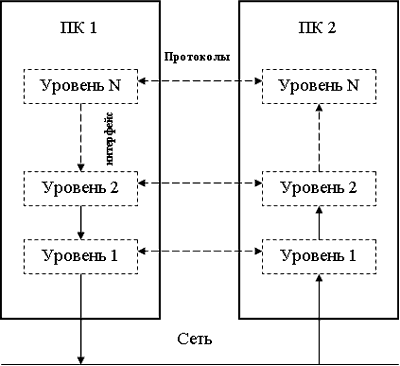
\includegraphics[width=200px]{01-proto_interface.png}
	\end{center}
\end{frame}

\begin{frame}{Протокол}
	\begin{center}
Уровень одной машины поддерживает связь с уровнем другой машины. 
Правила и соглашения, используемые в данном общении,  называются {\bfseries протоколом} уровня N.
	\end{center}
	\begin{center}
С сетевой точки зрения В протокол включаются форматы обмена данными (кадры,  сообщения) и правила обмена данными (последовательность)
	\end{center}
	\begin{center}
Протоколы могут меняться,  при условии,  что предоставляемые ими сервисы останутся неизменными.
	\end{center}
	\begin{center}
		Список протоколов,  используемых системой,  по одному протоколу на уровень,  называется {\bfseries стеком протоколов}.
	\end{center}
\end{frame}

\begin{frame}{Интерфейс}
	\begin{center}
		Между парой смежных уровней находится {\bfseries интерфейс}(служба),  определяющий набор примитивных операций,  предоставляемых нижним уровнем верхнему.
	\end{center}
	\begin{center}
	Когда разработчики решают,  сколько уровней включать в сеть и что должен делать каждый уровень,  одной из важнейших задач является определение ясных интерфейсов между ними. Эта задача требует,  чтобы каждый уровень выполнял особый набор хорошо понятных функций. Служба описывает интерфейс между двумя уровнями, где нижний уровень является поставщиком сервиса, а верхний – потребителем.
	\end{center}
\end{frame}

\begin{frame}{Архитектура сети}
	Набор уровней и протоколов называется {\bfseries архитектурой сети}.
	Спецификация архитектуры должна содержать достаточно информации для написания программного обеспечения и создания аппаратуры для каждого уровня,  чтобы они выполняли требования протокола. Детали реализации и спецификации интерфейсов не являются частями архитектуры,  поскольку они спрятаны внутри машины. При этом не требуется,  чтобы интерфейсы были одинаковыми,  главное,  чтобы протоколы соответствовали спецификации.
\end{frame}

\begin{frame}{Типы служб}
Уровни  могут предоставлять вышестоящим уровням услуги 2-х типов: с наличием или отсутствием соединения.
При наличии соединения клиент сначала устанавливает соединение,  а в конце разрывает его.
При отсутствии соединения клиент просто отсылает свое сообщение,  в котором содержится полный адрес получателя,  при этом каждое сообщение может идти своим путем и порядок получения данных не гарантируется.
\end{frame}

\begin{frame}{Службы ориентированные на соединение}
	\begin{itemize}
		\item Надежный поток сообщений
		\item Надежный поток байт
		\item Ненадежное соединение
	\end{itemize}
\end{frame}

\begin{frame}{Службы без установки соединения}
	\begin{itemize}
		\item Ненадежная дейтаграмма
		\item Дейтаграмма с подтверждением
		\item Запрос-Ответ
	\end{itemize}
\end{frame}

\begin{frame}{Примитивы служб}
	Служба формально описывается набором примитивов или операций,  доступных пользователю или другой сущности для получения сервиса. Эти примитивы заставляют службу выполнять некоторые действия или служат ответами на действия сущности такого же уровня. Если набор протоколов входит в состав ОС,  то примитивы являются системными вызовами.
\end{frame}

\begin{frame}{Примитивы служб}
	Набор примитивов может быть разным и зависит от типа предоставляемого сервиса. Например,  минимальный набор примитивов для простой передачи с установлением соединения будет выглядеть так:
	\begin{itemize}
		\item LISTEN (ожидание) -- ожидание входящего соединения
		\item CONNECT (соединение) -- установка соединенияс ожидающей сущностью такого же уровня
		\item RECEIVE (прием) -- ожидание входящего сообщения
		\item SEND (передача) -- отправка сообщения сущности того же уровня
		\item DISCONNECT (разрыв) -- разрыв соединения
	\end{itemize}
\end{frame}


\subsection{Проблемы при разработке стека протоколов}
\begin{frame}{Проблемы при разработке стека протоколов}
	Некоторые из ключевых аспектов разработки,  возникающих при создании компьютерных сетей,  присутствуют на нескольких уровнях.
\end{frame}

\begin{frame}{Адресация}
	Каждый уровень нуждается в механизме идентификации отправителей и получателей,  следовательно необходима система адресации.
\end{frame}

\begin{frame}{Логические каналы}
	Протокол должен определять количество логических каналов,  относящихся к соединению,  а также их приоритеты. Так,  многие сети обеспечивают как минимум два канала на соединение: один для обычных данных,  другой – для срочных.
\end{frame}

\begin{frame}{Контроль над ошибками}
	В протоколе должен быть предусмотрен контроль над ошибками. Получатель должен иметь возможность сообщить отправителю,  какие из сообщений были получены неправильно.
\end{frame}

\begin{frame}{Нумерация}
	Некоторые каналы связи (ориентированные на коммутацию пакетов) могут доставлять сообщения не в порядке отправления,  поэтому протокол должен явно снабжать сообщение номерами,  чтобы их можно было собрать в правильном порядке.
\end{frame}

\begin{frame}{Управление потоком}
	Также возникает вопрос: что делать,  чтобы более быстрая сторона не завалила своими пакетами более медленную ? Одно из решений – контроль состояния сторон,  другое решение – договоренность по ограничению скорости передачи между сторонами. В целом это называется управлением потоком.
\end{frame}

\begin{frame}{Размер сообщений}
Еще одна проблема возникает с размерами сообщений: что делать с огромными сообщениями и очень малыми,  которые неэффективно пересылать?
Например -- разбивать пакет на много малых либо наоборот.
\end{frame}

\begin{frame}{Мультиплексирование}
	Иногда неэффективно или невозможно установить отдельное соединение для каждой пары общающихся процессов,  тогда нижестоящий уровень может принять решение использовать одно и то же соединение для передачи нескольких соединений несвязанных между собой. Это называется уплотнением каналов или мультиплексированием и происходит прозрачно для вышестоящих уровней.
\end{frame}

\begin{frame}{Маршрутизация}
	Бывает так,  что между отправителем и получателем существует несколько путей следования сообщений,  в этом случае возникает проблема выбора оптимального пути. Эта задача маршрутизации.
\end{frame}


\end{document}
%Конец файла
